\documentclass[11pt]{scrartcl}

\usepackage[top=1in, bottom=2cm, left=1in, right=1in]{geometry}
\usepackage{graphicx}
\usepackage{amsmath}

\begin{document}

\title{HW4 STAT5376}
\subtitle{Dynamic programming}
\author{Li Sun}
\date{\today}
\maketitle

\noindent
To demonstrate the dynamic programming, I simulated several pairs of functions and try to register them.\\
1.First to register two identical function.\\
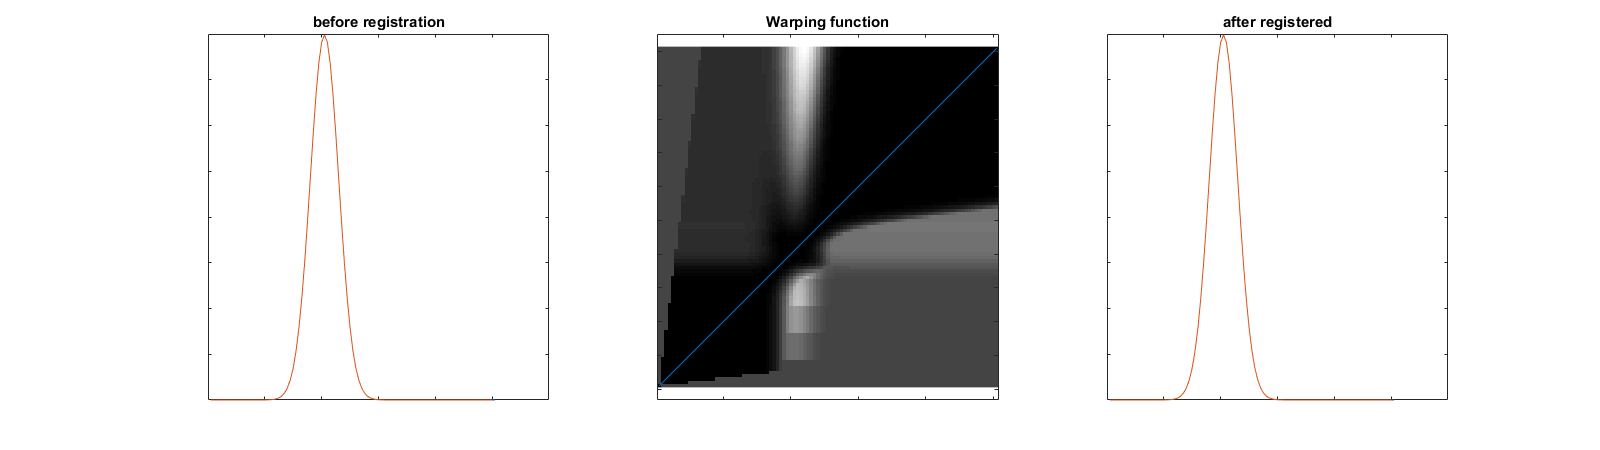
\includegraphics[scale=0.4]{hw41.png}\\
2.Register 2 functions with different locations but exact same shapes\\
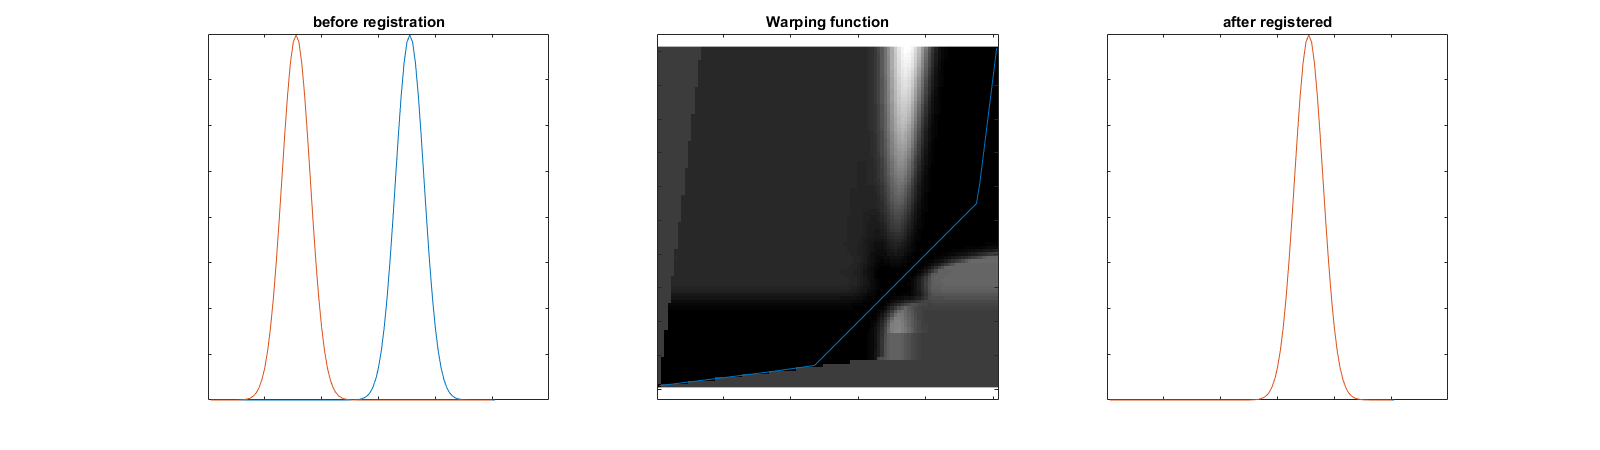
\includegraphics[scale=0.4]{hw42.png}\\
3.Functions with different variation but same location.\\
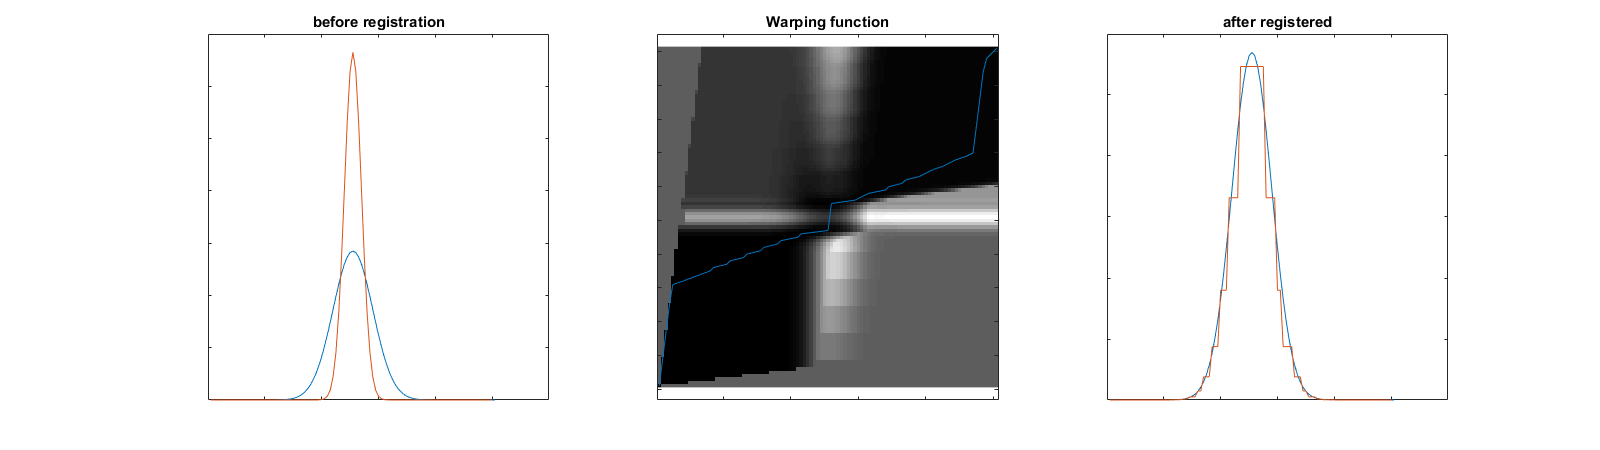
\includegraphics[scale=0.4]{hw43.png}\\
4.Functions with different center and different variations.\\
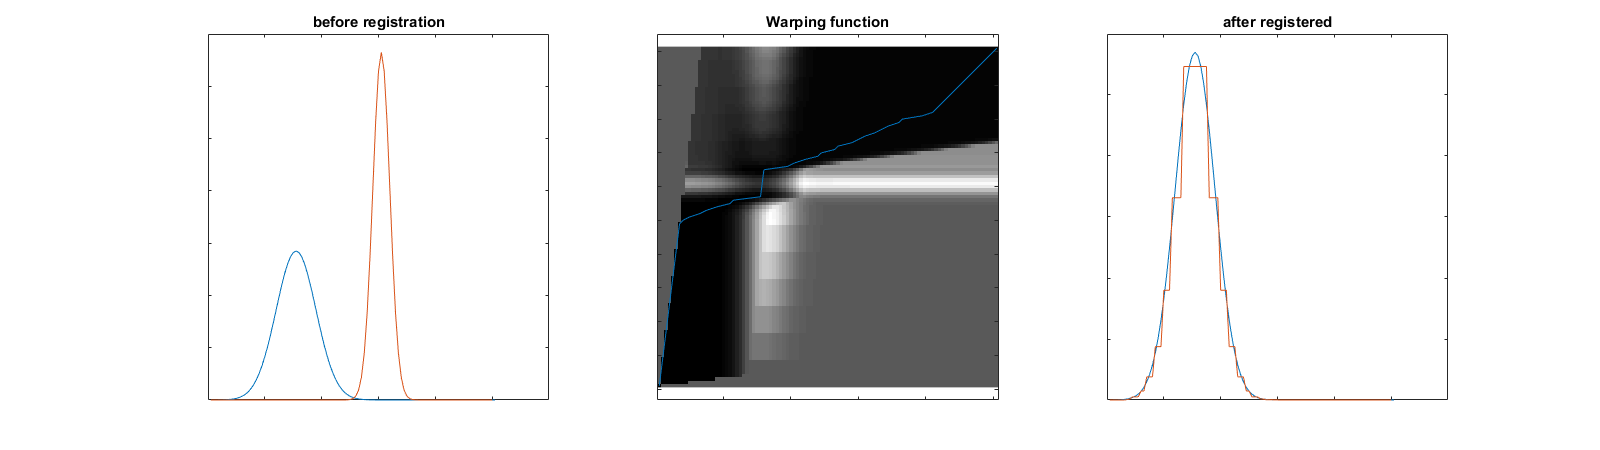
\includegraphics[scale=0.4]{hw44.png}\\
5.Let's try warp bi-peak function to function with only one peak.\\
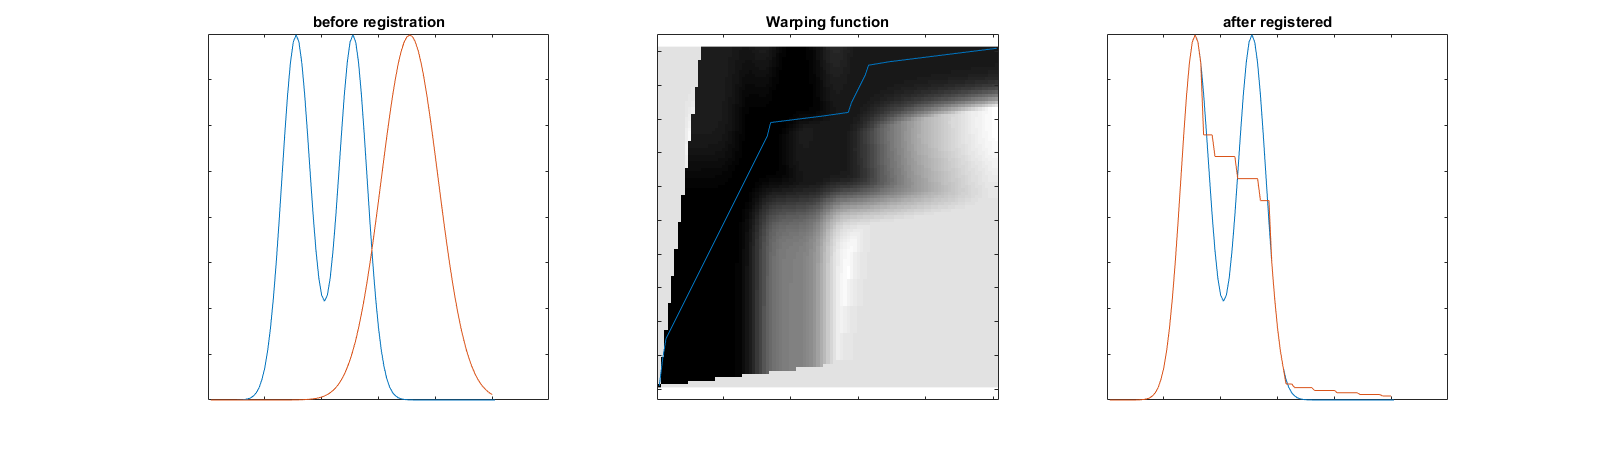
\includegraphics[scale=0.4]{hw45.png}\\
6. Two peak to Two peak.\\
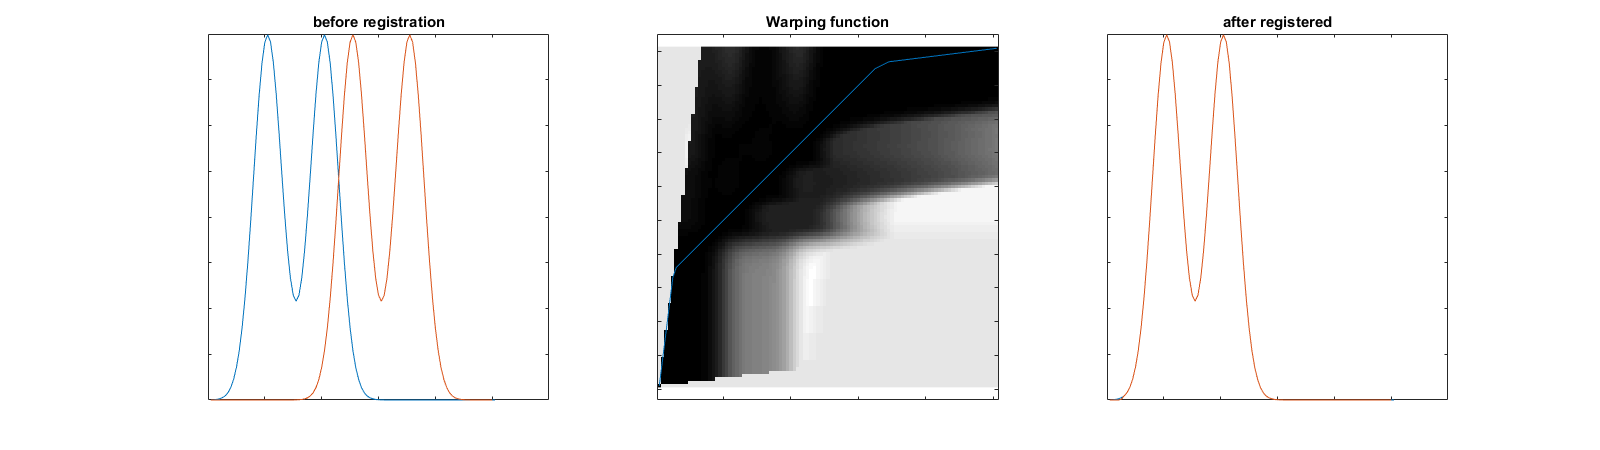
\includegraphics[scale=0.4]{hw46.png}\\

Above all, the algorithm searches 43 points as neighbors with 21 different slopes. It calculate fast and works well under most situations.\\
However, when function magnitude is different, it distorted function's shape. This might be due to the usage of L2 norm.\\

All code please see https://github.com/rikku1983/STAT5376\\
\bigskip

Thanks!


\end{document}